\chapter{System Theory and Design Fundamentals}

The proposed Visual Inspection of Solar Farm system integrates multiple engineering domains including drone technology, computer vision, deep learning, image processing, embedded systems, and web-based monitoring platforms. The effective functioning of such a system depends on a clear understanding of the theoretical principles governing image acquisition, fault detection, machine learning, and intelligent monitoring systems. This chapter elaborates on the fundamental concepts required for the design and development of the system, including visual inspection techniques, deep learning-based fault detection, drone-assisted monitoring, and system integration. These concepts collectively form the backbone of the system and enable efficient and intelligent inspection of solar farms.

\section{Visual Inspection Fundamentals}

Visual inspection is one of the most commonly used methods for identifying physical defects in photovoltaic panels and electrical infrastructure. It involves capturing high-resolution RGB images and analyzing them to detect abnormalities such as cracks, dust accumulation, bird droppings, shading effects, and damaged connectors.

\begin{figure}[H]
\centering
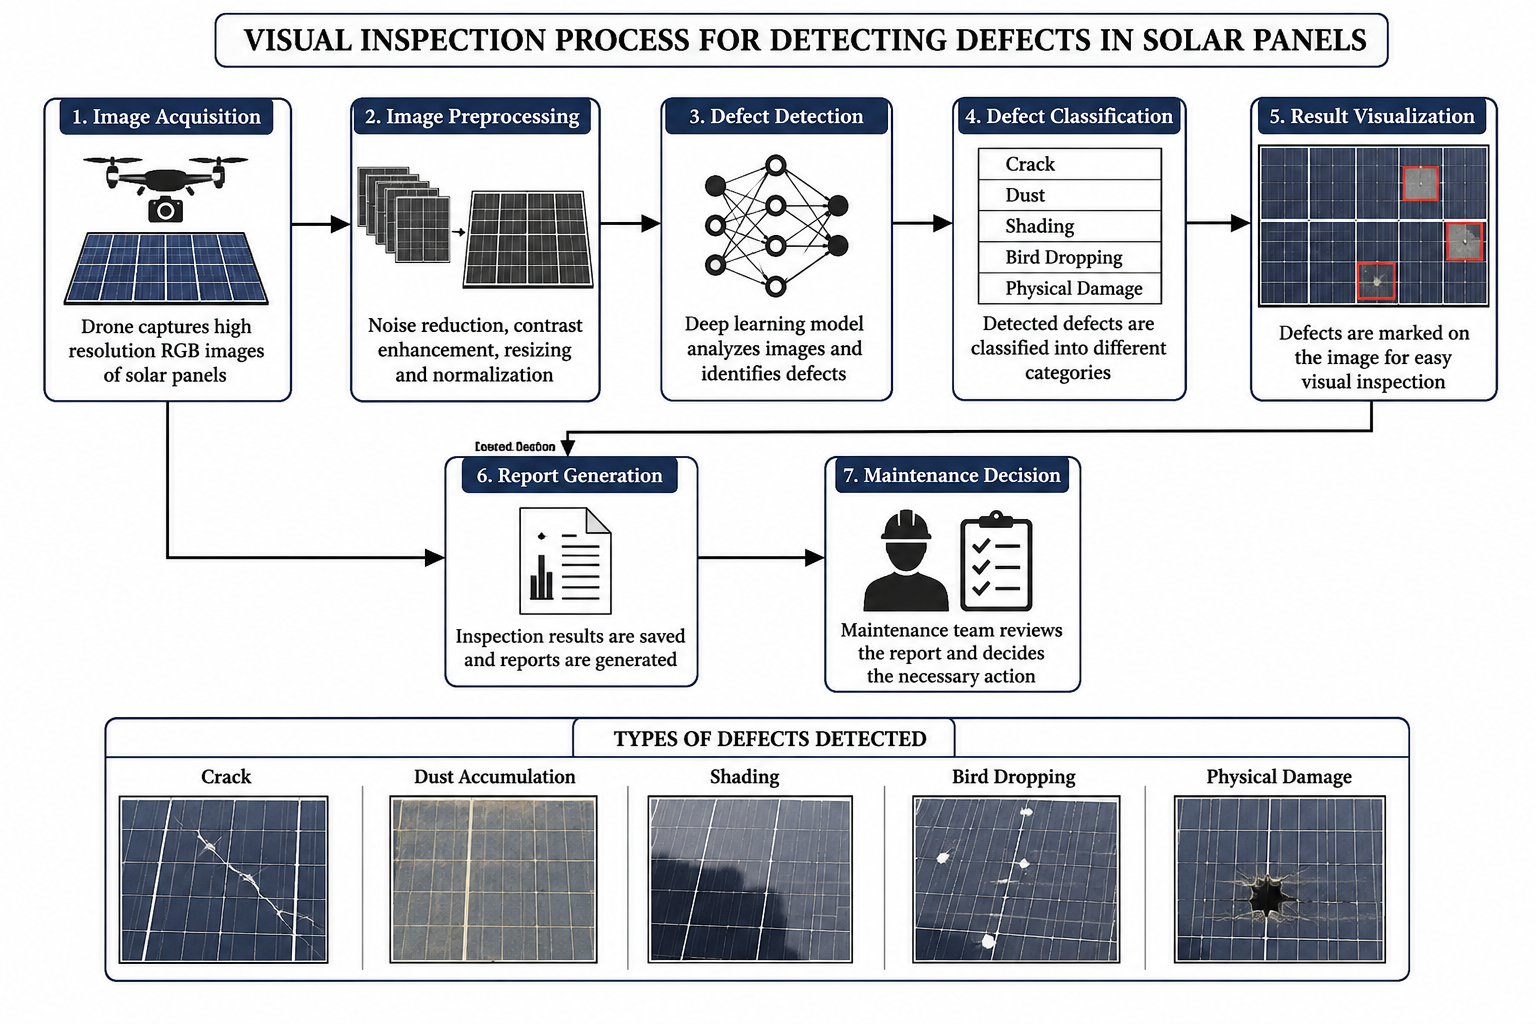
\includegraphics[width=0.7\textwidth]{figure/2.1.png}
\caption{Visual inspection process for detecting defects in solar panels}
\label{fig:visualinspection}
\end{figure}

As shown in Fig.~\ref{fig:visualinspection}, the visual inspection process begins with image acquisition, followed by image preprocessing, defect detection, classification, and report generation. This workflow enables automated identification of solar panel defects without requiring extensive manual inspection.

The effectiveness of visual inspection depends on image quality, environmental conditions, and the ability of image processing algorithms to identify fault patterns accurately.

Computer vision techniques enable automatic extraction of features from images and assist in identifying defects that may not be easily visible during manual inspections. Automated visual inspection improves efficiency, reduces human effort, and ensures consistent monitoring across large solar installations.

\subsection{Working Principle}

The visual inspection process begins with image acquisition using high-resolution RGB cameras mounted on drones. The captured images are transmitted to the processing unit where image enhancement and preprocessing operations are performed.

Subsequently, computer vision and deep learning models analyze the images to identify visible defects. The detected faults are classified and stored for further analysis and maintenance planning.

\section{Solar Panel Defect Classification Fundamentals}

Solar panel defects can significantly affect energy generation efficiency and long-term system reliability. Common defects include dust accumulation, bird droppings, physical damage, electrical damage, snow coverage, and surface cracks.

The proposed system utilizes image-based analysis to classify these defects automatically using deep learning techniques. By analyzing visual characteristics present in RGB images, the model can differentiate between healthy and defective panels.

\subsection{Classification Principle}

The classification process is based on extracting relevant visual features from solar panel images and comparing them with patterns learned during model training.

The major defect categories considered in this project are:

\begin{itemize}
\item Clean Panels
\item Dusty Panels
\item Bird Drop Defects
\item Physical Damage
\item Electrical Damage
\item Snow Covered Panels
\end{itemize}

Accurate classification enables maintenance teams to prioritize corrective actions and improve overall system efficiency.

\section{Drone-Based Inspection Technology}

Unmanned Aerial Vehicles (UAVs), commonly known as drones, have revolutionized infrastructure inspection by enabling rapid data acquisition over large geographical areas.

\begin{figure}[H]
\centering
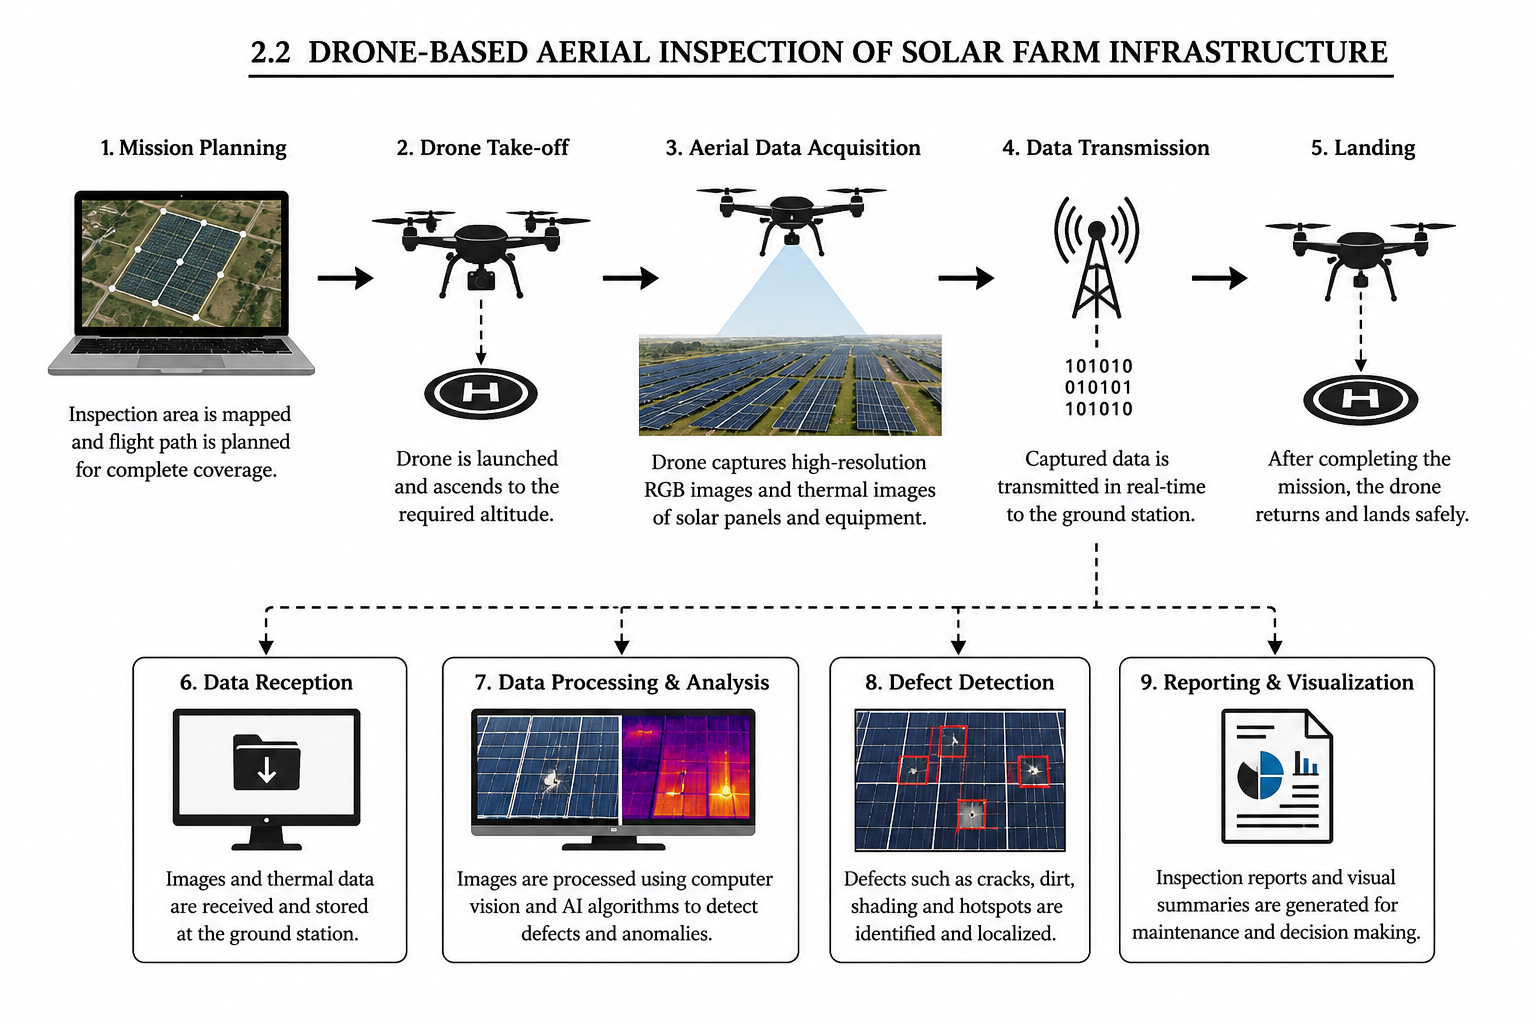
\includegraphics[width=0.6\textwidth]{figure/2.2.png}
\caption{Drone-based aerial inspection of solar farm infrastructure}
\label{fig:droneinspection}
\end{figure}

As illustrated in Fig.~\ref{fig:droneinspection}, drones perform systematic aerial surveys of solar farms and capture high-resolution RGB images of photovoltaic panels from multiple viewpoints. The collected images are then transferred for further processing and defect analysis.

Drone-assisted inspection offers several advantages:

\begin{itemize}
\item Rapid coverage of large installations
\item Reduced inspection time
\item Improved worker safety
\item High-quality data collection
\end{itemize}

The integration of drones with artificial intelligence enables automated monitoring and fault detection capabilities.

\section{Deep Learning-Based Fault Detection}

Deep learning has emerged as one of the most powerful approaches for image analysis and object detection. In this project, deep learning models are used to automatically identify defects present in solar panels.

Convolutional Neural Networks (CNNs) and object detection models such as YOLO are capable of learning complex visual patterns from large datasets and performing accurate fault classification.

\subsection{Working Principle}

The deep learning workflow involves:

\begin{itemize}
\item Dataset collection
\item Image annotation
\item Model training
\item Validation and testing
\item Real-time inference
\end{itemize}

During training, the model learns to recognize defect patterns from labeled images. Once trained, it can analyze new images and classify detected faults with high accuracy.

These models significantly reduce manual inspection efforts while improving detection consistency.

\section{Image Processing Techniques}

Image processing plays a crucial role in improving the quality of captured data before fault analysis.

\begin{figure}[H]
\centering
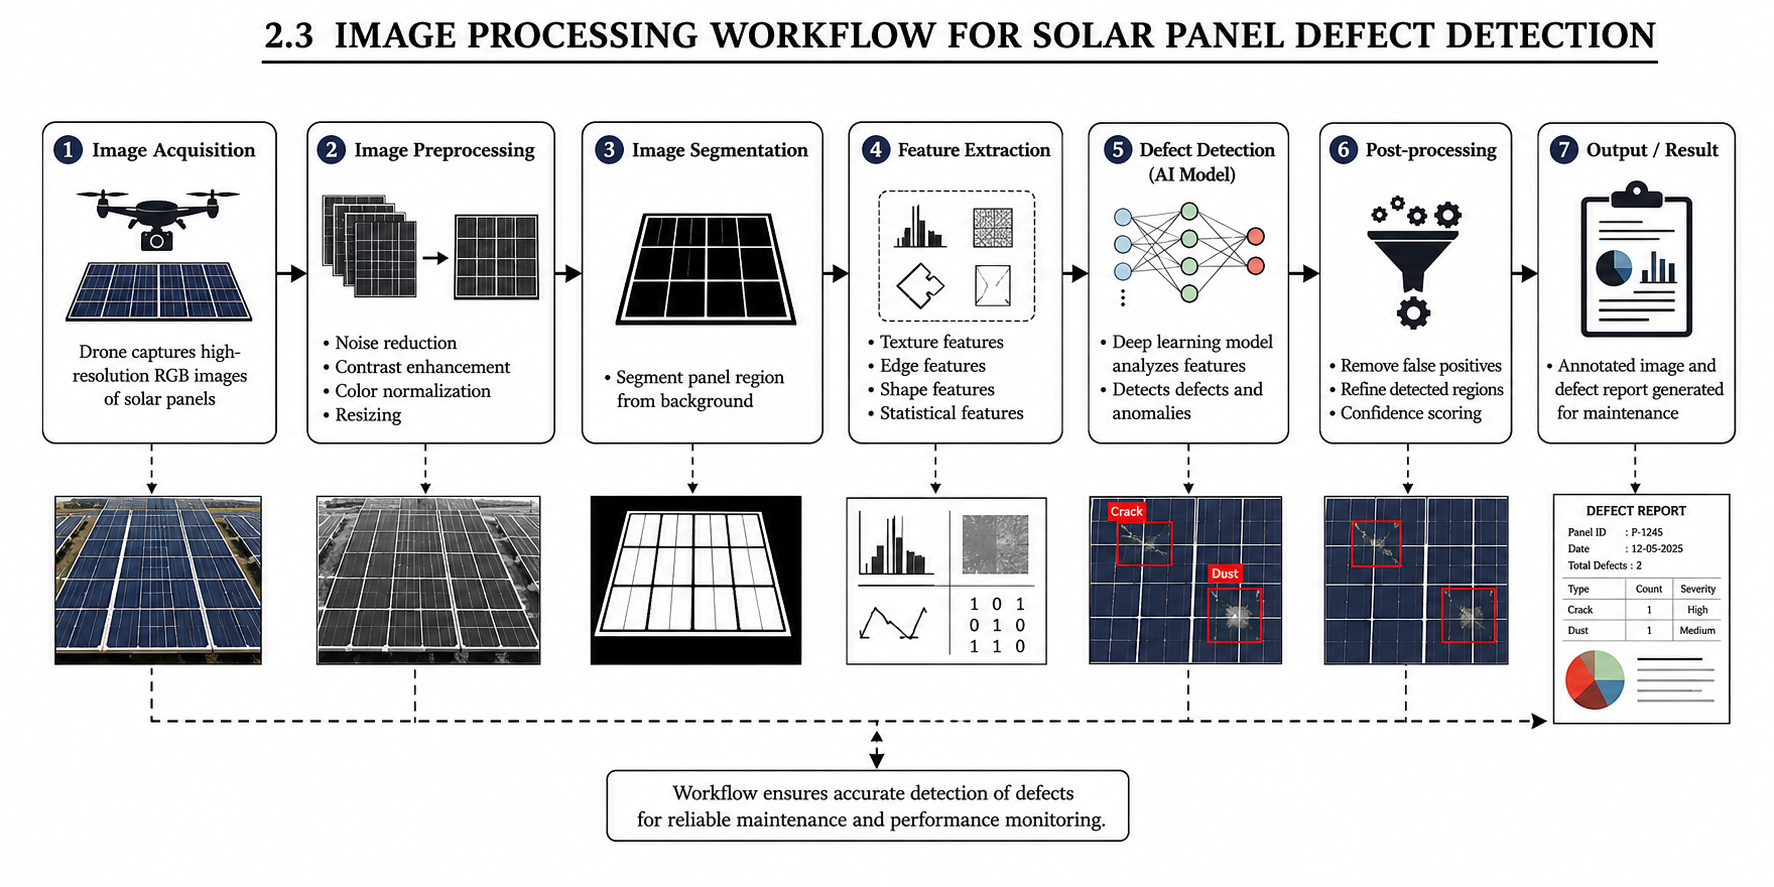
\includegraphics[width=0.7\textwidth]{figure/2.3.png}
\caption{Image processing workflow for solar panel defect detection}
\label{fig:imageprocessing}
\end{figure}

As shown in Fig.~\ref{fig:imageprocessing}, the image processing workflow consists of image acquisition, preprocessing, feature extraction, model inference, and defect classification. Each stage contributes to improving overall detection performance and model accuracy.

Common preprocessing operations include:

\begin{itemize}
\item Image resizing
\item Noise reduction
\item Contrast enhancement
\item Normalization
\item Feature extraction
\end{itemize}

These operations improve model performance and increase fault detection accuracy.

\section{Centralized Monitoring Platform}

The inspection system utilizes a centralized monitoring platform that stores inspection results and provides visualization tools for operators.

\subsection{Key Features}

\begin{itemize}
\item Real-time monitoring dashboard
\item Fault visualization and reporting
\item Historical inspection records
\item Maintenance recommendation generation
\end{itemize}

The platform enables operators to quickly identify critical issues and make informed maintenance decisions.

\subsection{Parameters Monitored}

\begin{itemize}
\item Panel health status
\item Fault category
\item Fault location
\item Inspection timestamps
\end{itemize}

These parameters help maintenance teams evaluate system performance and prioritize corrective actions.

\section{Embedded System Platform}

The system incorporates processing units responsible for image acquisition, image processing, and communication with centralized monitoring systems.

\subsection{Key Features}

\begin{itemize}
\item Real-time data acquisition
\item Image processing capability
\item Wireless communication support
\item Efficient resource utilization
\end{itemize}

The use of embedded processing platforms enables efficient operation and supports deployment in large-scale solar farm environments.

\section{Programming and Development Tools}

The development of the system involves both software and artificial intelligence components. Deep learning models, image processing modules, and monitoring platforms are developed using modern programming frameworks and tools.

\subsection{Software Development}

Python is primarily used for image processing, machine learning model development, and automation. Supporting libraries such as OpenCV and deep learning frameworks facilitate efficient implementation of fault detection algorithms.

\subsection{Development Environment}

The following tools are used:

\begin{itemize}
\item Python Programming Language
\item OpenCV Library
\item YOLO Deep Learning Framework
\item Drone Image Acquisition Software
\item Web Dashboard Development Tools
\end{itemize}

These tools provide development, testing, visualization, and deployment capabilities.

\section{System Integration Concept}

The system operates as an integrated platform where drones, cameras, processing units, artificial intelligence models, and monitoring dashboards work together in coordination. RGB images acquired during inspection are processed using computer vision algorithms and deep learning models. The generated results are transmitted to a centralized dashboard for visualization and reporting.

\begin{figure}[H]
\centering
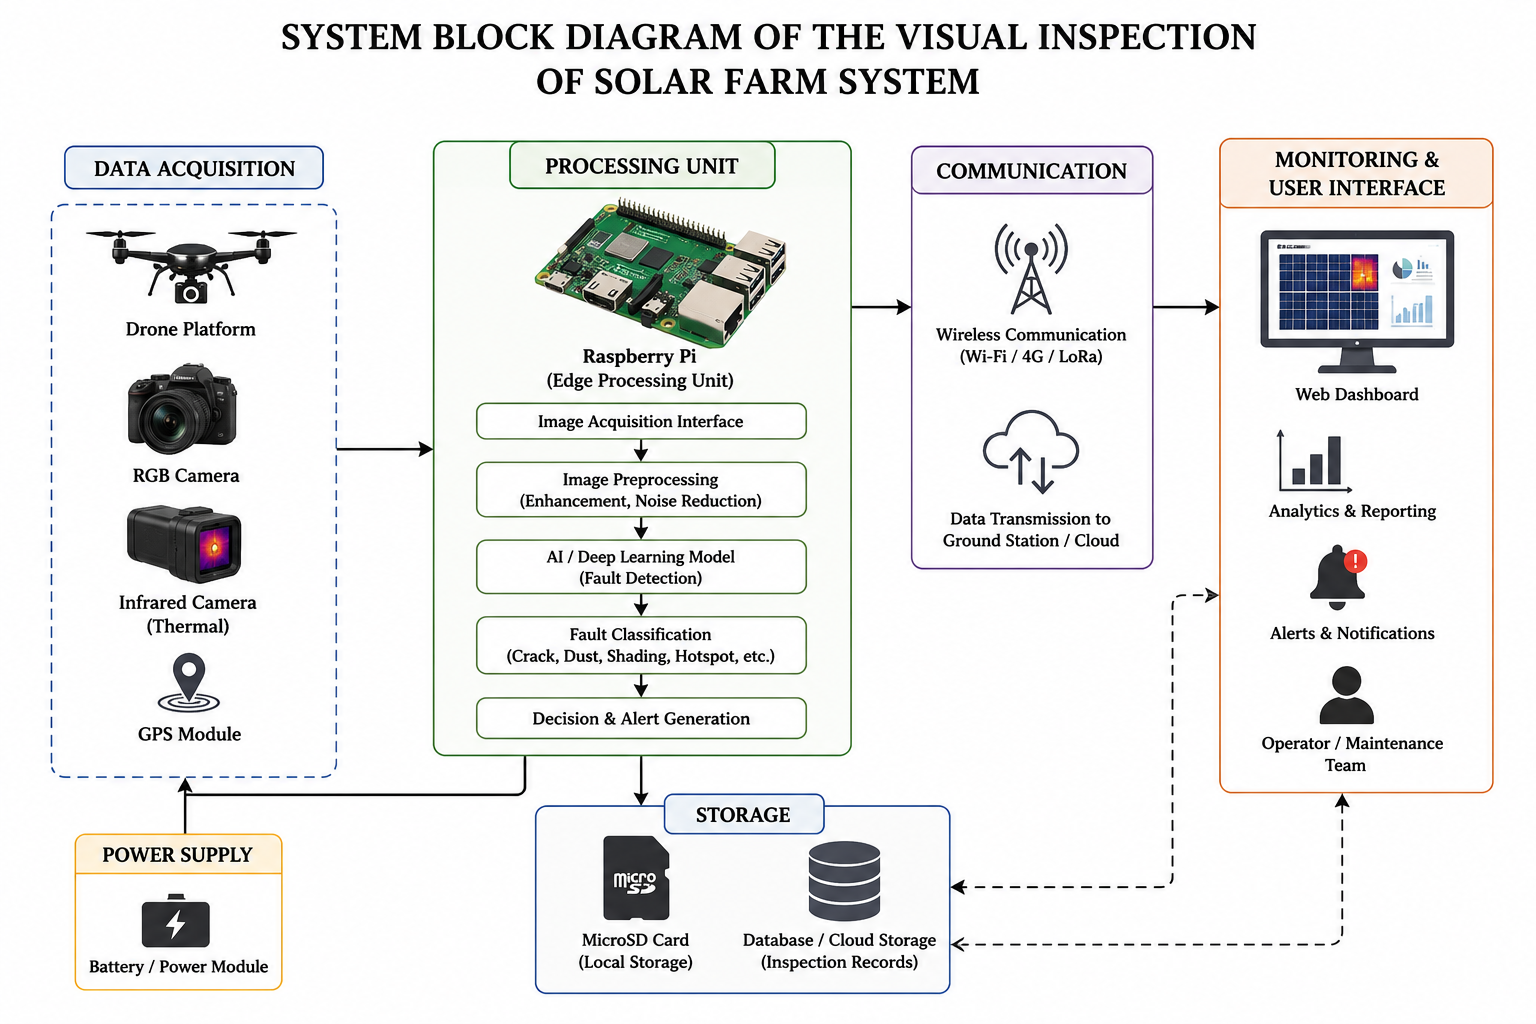
\includegraphics[width=0.8\textwidth]{figure/2.4.png}
\caption{System block diagram of the visual inspection of solar farm system}
\label{fig:block}
\end{figure}

As illustrated in Fig.~\ref{fig:block}, the system consists of five major components: image acquisition, image preprocessing, deep learning-based defect detection, database storage, and dashboard visualization. These modules operate together to provide automated inspection and maintenance support.

The integration of data acquisition, intelligent analysis, and monitoring capabilities enables autonomous inspection and efficient maintenance planning.

\section{Use of Acronyms and Glossaries}

Examples:

\begin{itemize}
\item UAV: Unmanned Aerial Vehicle
\item RGB: Red Green Blue
\item CNN: Convolutional Neural Network
\item YOLO: You Only Look Once
\end{itemize}

\section{Chapter Summary}

This chapter provided a detailed overview of the theoretical concepts and fundamental principles required for the development of the Visual Inspection of Solar Farm system. The concepts of visual inspection, solar panel defect classification, drone-based monitoring, deep learning-based fault detection, image processing, centralized monitoring, and system integration were discussed in detail. These concepts form the foundation for the design and implementation presented in the subsequent chapters.